% ==============================================================================
% PLANTILLA DE INFORME - PFM02 / IIIEPE / MAEM
% ==============================================================================
% Uso:
% 1. Duplica este archivo y renombra la copia por unidad, sesion y actividad.
% 2. Actualiza documenttitle, documentsubtitle, documentsubject, sesionname,
%    activityname, docente y fecha de entrega.
% 3. Lee la consigna del EVA/posgrado y NO pegues las instrucciones completas
%    dentro del producto final. Usa la consigna como lista de cumplimiento.
% 4. Revisa la bibliografia indicada, toma notas, registra citas y redacta con
%    comprension propia.
% 5. Identifica el producto academico o didactico solicitado y construyelo dentro
%    del documento siempre que sea posible.
% 6. Entrega en PDF con la nomenclatura indicada por la unidad de aprendizaje.
%
% Formato institucional recomendado para IIIEPE:
% - Fuente tipo Helvetica, equivalente visual a Arial.
% - Interlineado 1.5.
% - Citas autor-anio con natbib: usar \citep{clave} o \citet{clave}.
% - Referencias en bibliografia BibTeX, formato APA 7 en cuerpo y referencias.
% - Caratula, resumen breve, desarrollo, producto solicitado, conclusion y
%   bibliografia.
% - Redaccion academica clara, coherente, cohesionada, formal y sin faltas.
% - Portada con identidad IIIEPE, programa MAEM, matricula y correo institucional.
% - La portada puede llevar una marca de agua institucional discreta; ajustar
%   las variables coverwatermark... si se requiere apagarla o cambiar intensidad.
%
% Criterios generales de cumplimiento:
% - Responder exactamente a la actividad solicitada en el EVA o por la figura docente.
% - Alinear contenido matematico, PDA, aprendizaje de la secuencia, fases,
%   evaluacion y retroalimentacion.
% - Identificar conceptos, elementos, criterios o categorias de forma precisa.
% - Analizar, interpretar y tomar postura; no solo copiar fuentes.
% - Organizar la informacion por jerarquia, secuencia y criterios claros.
% - Incluir conclusion personal cuando la actividad lo permita o lo solicite.
% - Usar citas y referencias en APA 7.
% - Evitar copiar las indicaciones de la actividad en el cuerpo final.
%
% Regla para productos visuales:
% - Si la actividad pide tabla, cuadro comparativo, esquema, mapa conceptual,
%   mapa mental, linea de tiempo, diagrama, matriz, lista de verificacion, red
%   conceptual, SQA, organizador grafico o producto similar, realizarlo
%   preferentemente con LaTeX/TikZ para mantener nitidez, evidencia editable y
%   diseno controlado.
% - Si la consigna exige Canva, Miro u otra herramienta externa, insertar una
%   captura nitida y conservar la explicacion dentro del documento.
% - Para tablas extensas, usar pagina limpia, sin encabezados ni pies, landscape,
%   letra pequena y restaurar el estilo al terminar.
%
% Criterios de redaccion personal:
% - No escribir para llenar espacio; escribir para sostener una idea.
% - Convertir informacion en criterio: que significa, como funciona, que problema
%   resuelve, que limite presenta y que consecuencia produce.
% - Estructura mental recomendada: problema -> sistema -> consecuencia -> postura.
% - Usar pensamiento de diagnostico: entrada -> proceso -> salida.
% - Cada parrafo debe tener funcion: presentar, explicar, comparar, valorar o
%   concluir.
% - Usar primera persona con moderacion academica: "Considero que",
%   "Desde esta perspectiva", "La posicion que sostengo es". Evitar "yo creo".
%
% Notas de enfoque personal segun enfoque_personal.txt:
% - La voz debe ser academica, tecnica, directa, estrategica y funcional.
% - El texto no debe sonar como estudiante pasivo que recopila: debe sonar como
%   alguien que interpreta, ordena, cruza datos y busca consecuencia practica.
% - Antes de redactar, identificar la funcion de cada seccion: abrir problema,
%   definir criterio, demostrar con evidencia, comparar, valorar o concluir.
% - Evitar frases genericas como "es importante porque si" o "desde siempre".
%   Sustituirlas por relaciones verificables: causa, efecto, limite, costo,
%   funcion, riesgo, implicacion o mejora.
% - Cada concepto debe pasar de definicion a analisis. Formula util:
%   concepto -> funcion -> riesgo si se aplica mal -> consecuencia -> postura.
% - La postura personal no debe ser opinion suelta. Debe tener tres piezas:
%   posicion, razon y efecto. Ejemplo: "Considero que X, porque Y; por ello Z".
% - Integrar experiencia o criterio propio sin perder formalidad: no narrar la
%   vida personal, sino usar mirada practica para explicar por que el tema
%   importa en educacion, derecho, instituciones, comunicacion o profesion.
%
% Estilo observado en actividades ya realizadas:
% - Abrir con una tesis concreta:
%   "La ensenanza de las matematicas no solo transmite procedimientos:
%   organiza formas de razonar, representar y justificar."
% - Formular el problema en negativo y positivo:
%   "El problema no es solo..., sino..."
% - Convertir el producto visual en argumento:
%   "El cuadro no solo recopila datos; reconstruye la funcion, el problema y el
%   punto que requiere correccion."
% - Cerrar con aprendizaje transferible:
%   "No basta con saber que dice la norma; tambien debe analizarse a quien
%   protege, a quien excluye y que razones permiten defenderla publicamente."
%
% Nivel cognitivo esperado:
% - Recordar: usar solo para definir conceptos basicos. No debe ser el nivel
%   dominante en una actividad ponderable.
% - Comprender: explicar con palabras propias y relacionar con el tema.
% - Aplicar: llevar el concepto a un caso, norma, texto, correo, dilema o hecho.
% - Analizar: separar elementos, detectar causas, efectos, tensiones y limites.
% - Evaluar: sostener una postura con criterios, fuentes y consecuencias.
% - Crear: elaborar producto propio: mapa, cuadro, linea de tiempo, ensayo,
%   propuesta, reformulacion, glosario, portafolio o solucion argumentada.
%
% Regla de nivel minimo:
% - Si la actividad vale puntos y pide producto, no quedarse en recordar o
%   comprender. Debe llegar por lo menos a aplicar y analizar; si pide conclusion
%   o postura, debe llegar a evaluar.
%
% Uso de tecnicas didacticas:
% - Esta plantilla conserva el manual "Tecnicas didacticas del aprendizaje" como
%   apoyo para construir productos visuales, analiticos y reflexivos.
% - Cuando la actividad mencione una tecnica didactica, identificar: definicion
%   de la tecnica, producto esperado, pasos de construccion, criterios de revision
%   y cierre reflexivo.
% - La tecnica didactica no debe verse como adorno. Debe mostrar seleccion,
%   jerarquia, relacion entre ideas y lectura propia.
% - Siempre que sea viable, construir la tecnica en LaTeX/TikZ: cuadro
%   comparativo, mapa conceptual, esquema, mapa mental, linea de tiempo, matriz,
%   red conceptual, diagrama de flujo, tabla SQA o lista de verificacion.
%
% Checklist antes de entregar:
% [ ] El titulo, unidad de aprendizaje, sesion, docente y fecha estan actualizados.
% [ ] El objetivo coincide con la consigna del EVA/posgrado.
% [ ] El contenido, PDA y aprendizaje de la secuencia estan alineados.
% [ ] La actividad considera las cinco fases de PFM02 cuando se trate de una secuencia.
% [ ] La practica incluye mecanizacion, variacion y al menos una situacion en contexto.
% [ ] La evaluacion mide el aprendizaje declarado y no solo la repeticion del algoritmo.
% [ ] El producto solicitado aparece visible, rotulado y completo.
% [ ] La introduccion plantea un problema o postura, no solo anuncia el tema.
% [ ] El desarrollo explica, conecta y analiza.
% [ ] Hay citas APA autor-anio dentro del texto.
% [ ] La bibliografia final coincide con las fuentes citadas.
% [ ] La conclusion responde que se comprendio y que postura se sostiene.
% [ ] El nivel cognitivo llega al menos a aplicacion y analisis.
% [ ] Si hay conclusion/postura, incluye posicion, razon y consecuencia.
% [ ] La tecnica didactica solicitada esta construida y explicada.
% [ ] No aparecen instrucciones copiadas de la consigna dentro del producto.
% [ ] Ortografia, acentos, sintaxis y nombres propios revisados.
% [ ] Si se uso IA como apoyo, el texto fue comprendido, revisado y apropiado.
% ==============================================================================

% CREACION DEL DOCUMENTO
\documentclass[
	spanish,
	letterpaper, oneside
]{article}

% ==============================================================================
% INFORMACION DEL DOCUMENTO
% Actualizar en cada actividad.
% Ejemplos:
% \def\documenttitle {Multiplicacion y division con fracciones}
% \def\documentsubtitle {Actividad X - Nombre de la asignatura}
% \def\documentsubject {Sesion 03 -- Secuencia didactica con solucion de actividades}
% ==============================================================================
\def\documenttitle {Multiplicacion y division con fracciones}
\def\documentsubtitle {PFM02 - Temas selectos de matematicas I}
\def\documentsubject {Sesion 03 -- Secuencia didactica con solucion de actividades}

\def\documentauthor {Mtro. Martin Jonathan de la Cruz Munoz}
\def\coursename {Temas selectos de matematicas I}
\def\coursecode {PFM02}

\def\universityname {Instituto de Investigacion, Innovacion y Estudios de Posgrado para la Educacion \\ del Estado de Nuevo Leon}
\def\universityfaculty {Maestria en Aprendizaje y Ensenanza de las Matematicas}
\def\universitydepartment {Temas selectos de matematicas I}
\def\universitydepartmentimage {img/iiiepe/marca-iiiepe.png}
\def\universitydepartmentimagecfg {height=1.75cm}
\def\universitylocation {Monterrey, Nuevo Leon}

% DATOS FIJOS DEL POSGRADO
\def\studentfullname {Mtro. Martin Jonathan de la Cruz Munoz}
\def\studentid {00841}
\def\studentemail {martin.delacruz@campus.iiiepe.edu.mx}
\def\institutionurl {https://iiiepe.edu.mx/}
\def\programperiod {1er tetramestre marzo--julio 2026}
\def\programmodality {Modalidad presencial}
\def\programshort {MAEM}
\def\maemsource {https://iiiepe.edu.mx/maestria-en-aprendizaje-y-ensenanza-de-las-matematicas/}
\def\coursegroup {Grupo A}
\def\courseperiod {Marzo--julio 2026}
\def\evaname {EVA posgrado}
\def\activityname {S03 -- Multiplicacion y division con fracciones}
\def\sessionname {Sesion 03}
\def\blockname {Bloque 1: Numeros racionales y operaciones}
\def\methodology {Aprendizaje basado en indagacion}
\def\steamenfoque {STEAM como enfoque}
\def\curriculumsource {Programa Sintetico Fase 6}
\def\formativefield {Saberes y Pensamiento Cientifico}
\def\mainproduct {Informe academico con secuencia didactica matematica}
\def\docentename {Mtro. Jonathan Cardenas (Coordinador PFM02)}

% INTEGRANTES, PROFESORES Y FECHAS
\def\authortable {
	\begin{tabular}{ll}
		\textbf{Alumno:}
		& \begin{tabular}[t]{l}
			 \studentfullname \\
		\end{tabular} \\
		Matricula: & \studentid \\
		Correo institucional: & \studentemail \\

		\textit{Figura docente:}
		& \begin{tabular}[t]{l}
			\docentename
		\end{tabular} \\
		Unidad: & \coursename \\
		Clave: & \coursecode \\
		Grupo: & \coursegroup \\
		Sesion/Bloque: & \sessionname\ / \blockname \\
		Actividad: & \activityname \\
		Programa: & \programshort \\
		Periodo: & \courseperiod \\
		& \\
		\multicolumn{2}{l}{Fecha de realizacion: \today} \\
		\multicolumn{2}{l}{\universitylocation}
	\end{tabular}
}

% IMPORTACION DEL TEMPLATE BASE
\input{template}

% FORMATO GENERAL
\usepackage{helvet}
\renewcommand{\familydefault}{\sfdefault}

% IDENTIDAD VISUAL IIIEPE
\definecolor{iiiepeNavy}{HTML}{163B5C}
\definecolor{iiiepeBlue}{HTML}{1F6F9F}
\definecolor{iiiepeAqua}{HTML}{20B7A8}
\definecolor{iiiepeOrange}{HTML}{F28C28}
\definecolor{iiiepePaper}{HTML}{F6F8F7}
\definecolor{iiiepeInk}{HTML}{1E2A32}
\definecolor{iiiepeMuted}{HTML}{667085}
\def\portraittitlecolor {iiiepeNavy}

% TABLAS Y PRODUCTOS VISUALES
\usepackage{array}
\usepackage{tabularx}
\usepackage{makecell}
\usepackage{longtable}
\usepackage{etoolbox}
\usepackage{pdflscape}
\usepackage{textcomp}
\usepackage{tikz}
\setlength{\LTcapwidth}{\textwidth}
\makeatletter
\newcommand{\PFMTableSetup}{%
	\ifdim\f@size pt>9.1pt\small\fi
	\renewcommand{\arraystretch}{1.35}%
	\setlength{\tabcolsep}{4pt}%
	\rowcolors{2}{gray!10}{white}%
}
\AtBeginEnvironment{longtable}{\PFMTableSetup}
\AtEndEnvironment{longtable}{\rowcolors{2}{}{}}
\makeatother
\usetikzlibrary{
	arrows.meta,
	positioning,
	calc,
	matrix,
	fit,
	shapes.geometric,
	decorations.pathreplacing,
	shadows.blur
}

\newcommand{\DividirEntre}[2]{\ensuremath{#1\,\text{ entre }\,#2}}
\newcommand{\signodiv}{\mathbin{\text{\normalfont\textdiv}}}

\tikzset{
	cajaProc/.style={
		draw=iiiepeBlue,
		rounded corners=2mm,
		align=center,
		inner sep=5pt,
		minimum height=8mm,
		font=\small
	},
	cajaDato/.style={
		cajaProc,
		fill=iiiepeBlue!8
	},
	cajaOp/.style={
		cajaProc,
		fill=iiiepeOrange!12
	},
	cajaRes/.style={
		cajaProc,
		fill=iiiepeAqua!12
	},
	flechaProc/.style={
		-{Latex[length=2.5mm]},
		thick,
		draw=iiiepeBlue
	},
	notaProc/.style={
		draw=iiiepeOrange,
		rounded corners=2mm,
		fill=iiiepeOrange!12,
		align=center,
		inner sep=4pt,
		font=\scriptsize
	},
	decisionProc/.style={
		diamond,
		aspect=2.1,
		draw=iiiepeBlue,
		fill=iiiepeAqua!10,
		align=center,
		inner sep=2pt,
		font=\scriptsize
	}
}

\newcommand{\RutaOperacion}[4]{%
\begin{tikzpicture}[node distance=8mm]
	\node[cajaDato] (a) {#1};
	\node[cajaOp, right=of a] (b) {#2};
	\node[cajaOp, right=of b] (c) {#3};
	\node[cajaRes, right=of c] (d) {#4};
	\draw[flechaProc] (a) -- (b);
	\draw[flechaProc] (b) -- (c);
	\draw[flechaProc] (c) -- (d);
\end{tikzpicture}%
}

\newcommand{\RutaOperacionCinco}[5]{%
\begin{tikzpicture}[node distance=7mm]
	\node[cajaDato] (a) {#1};
	\node[cajaOp, right=of a] (b) {#2};
	\node[cajaOp, right=of b] (c) {#3};
	\node[cajaOp, right=of c] (d) {#4};
	\node[cajaRes, right=of d] (e) {#5};
	\draw[flechaProc] (a) -- (b);
	\draw[flechaProc] (b) -- (c);
	\draw[flechaProc] (c) -- (d);
	\draw[flechaProc] (d) -- (e);
\end{tikzpicture}%
}

\newcommand{\GridProducto}[5]{%
\begin{tikzpicture}[scale=#5]
	\pgfmathsetmacro{\yini}{#4-#3}
	\pgfmathsetmacro{\xmitad}{#1/2}
	\pgfmathsetmacro{\ymitad}{#4-#3/2}
	\pgfmathsetmacro{\yarriba}{#4+0.22}
	\pgfmathsetmacro{\xderecha}{#2+0.18}
	\fill[iiiepeBlue!18] (0,0) rectangle (#1,#4);
	\fill[iiiepeOrange!18] (0,\yini) rectangle (#2,#4);
	\fill[iiiepeAqua!55] (0,\yini) rectangle (#1,#4);
	\draw[step=1,gray!55,very thin] (0,0) grid (#2,#4);
	\draw[thick] (0,0) rectangle (#2,#4);
	\draw[decorate,decoration={brace,mirror,raise=3pt}] (0,-0.08) -- (#2,-0.08)
		node[midway,below=6pt] {\scriptsize #2 partes};
	\draw[decorate,decoration={brace,raise=3pt}] (-0.08,0) -- (-0.08,#4)
		node[midway,left=6pt] {\scriptsize #4 partes};
	\node[above] at (\xmitad,\yarriba) {\scriptsize #1 tomadas};
	\node[right] at (\xderecha,\ymitad) {\scriptsize #3 tomadas};
\end{tikzpicture}%
}

% CITAS EN FORMATO AUTOR-ANIO, COMPATIBLE CON APA 7 EN EL CUERPO DEL TEXTO
% Usar:
% - Cita parentetica: \citep{clave}
% - Cita narrativa: \citet{clave}
% - Varias fuentes: \citep{clave1,clave2}
\setcitestyle{authoryear,open={(},close={)}}

% ==============================================================================
% AYUDAS DE REDACCION
% Quitar o comentar \pendiente cuando el documento final este terminado.
% ==============================================================================
\newcommand{\pendiente}[1]{\textcolor{red}{[PENDIENTE: #1]}}

% ==============================================================================
% MARCA DE AGUA EN PORTADA
% - Se aplica solo a la portada porque usa \AddToShipoutPictureBG*.
% - Para apagarla en alguna actividad: \def\coverwatermarkenabled {false}
% - Usar opacidad baja para que no compita con titulo, datos ni logotipo.
% ==============================================================================
\def\coverwatermarkenabled {true}
\def\coverwatermarkimage {img/iiiepe/logo-puntos.png}
\def\coverwatermarkopacity {0.09}
\def\coverwatermarkwidth {0.58\paperwidth}
\def\coverwatermarkxshift {0cm}
\def\coverwatermarkyshift {-0.15cm}

\newcommand{\insertcoverwatermark}{%
	\ifthenelse{\equal{\coverwatermarkenabled}{true}}{%
		\AddToShipoutPictureBG*{%
			\begin{tikzpicture}[remember picture,overlay]
				\node[
					opacity=\coverwatermarkopacity,
					inner sep=0pt,
					xshift=\coverwatermarkxshift,
					yshift=\coverwatermarkyshift
				] at (current page.center) {%
					\includegraphics[width=\coverwatermarkwidth]{\coverwatermarkimage}%
				};
			\end{tikzpicture}%
		}%
	}{}%
}

\begin{document}

% PORTADA
\insertcoverwatermark
\templatePortrait

% CONFIGURACION DE PAGINA Y ENCABEZADOS
\templatePagecfg
\onehalfspacing

% ==============================================================================
% RESUMEN / ABSTRACT
% Debe ser breve. Formula recomendada:
% Tema + objetivo + tecnica/producto + enfoque personal.
% ==============================================================================
\begin{abstractd}
	\textbf{Objetivo:} Actualizar la actividad de la Sesion 03 para resolver y explicar procedimientos de multiplicacion y division con fracciones, integrando la estructura institucional de secuencia didactica y los criterios generales de evaluacion del curso.

	\textbf{Contenido:} Extension del significado de las operaciones y sus relaciones inversas.

	\textbf{PDA:} Reconoce el significado de las cuatro operaciones basicas y sus relaciones inversas al resolver problemas que impliquen el uso de numeros con signo.

	\textbf{Aprendizaje de la secuencia:} Resolver situaciones problematicas que involucran multiplicar o dividir fracciones.

	\textbf{Producto:} Reporte academico con procedimientos explicitos, ejercicios resueltos, situaciones contextualizadas, autoevaluacion y retroalimentacion.
\end{abstractd}

% TABLA DE CONTENIDOS - INDICE
\templateIndex

% CONFIGURACIONES FINALES
\templateFinalcfg

% ======================= INICIO DEL DOCUMENTO =======================

\section{Introduccion}

La multiplicacion y la division con fracciones exigen ampliar el sentido habitual de las operaciones. Multiplicar ya no significa siempre ``hacer mas'', porque multiplicar por una fraccion menor que la unidad puede representar tomar una parte de otra parte. Del mismo modo, dividir no solo significa repartir en partes iguales, sino tambien preguntar cuantas porciones de cierto tamano caben en una cantidad dada.

Esta actividad se organiza conforme a la estructura institucional de la secuencia didactica de PFM02: antecedente del contenido, introduccion y explicacion, practica, evaluacion y retroalimentacion. Tambien toma en cuenta los criterios generales de evaluacion del curso, donde las actividades diarias, la exposicion de secuencias, el escrito reflexivo y la exposicion final deben mostrar claridad conceptual, procedimiento visible, aplicacion contextual y reflexion sobre el aprendizaje.

El enfoque del reporte es pedagogico y operativo. Cada procedimiento muestra la estrategia, el desarrollo, la simplificacion y la interpretacion contextual. Asi, las soluciones no quedan como una lista de respuestas, sino como evidencias de razonamiento transferible a problemas de area, capacidad, reparto, deuda, medida y consumo.

\section{Desarrollo de la actividad}

\subsection{Datos base de la secuencia}

\begin{longtable}{@{}p{0.28\linewidth}p{0.65\linewidth}@{}}
	\caption{Datos institucionales de la Sesion 03}\label{tab:datos-sesion03}\\
	\toprule
	\textbf{Elemento} & \textbf{Descripcion} \\
	\midrule
	\endfirsthead
	\toprule
	\textbf{Elemento} & \textbf{Descripcion} \\
	\midrule
	\endhead
	Tema & Multiplicacion y division con fracciones. \\
	Contenido & Extension del significado de las operaciones y sus relaciones inversas. \\
	Proceso de desarrollo de aprendizaje & Reconoce el significado de las cuatro operaciones basicas y sus relaciones inversas al resolver problemas que impliquen el uso de numeros con signo. \\
	Aprendizaje de la secuencia & Resolver situaciones problematicas que involucran multiplicar o dividir fracciones. \\
	Producto esperado & Procedimientos escritos, ejercicios resueltos, situaciones en contexto, autoevaluacion y retroalimentacion. \\
	\bottomrule
\end{longtable}

\subsection{Criterios institucionales incorporados}

\begin{longtable}{@{}p{0.26\linewidth}p{0.32\linewidth}p{0.34\linewidth}@{}}
	\caption{Traduccion de criterios institucionales al producto elaborado}\label{tab:criterios-institucionales-s03}\\
	\toprule
	\textbf{Fuente institucional} & \textbf{Criterio recuperado} & \textbf{Aplicacion en este reporte y presentacion} \\
	\midrule
	\endfirsthead
	\toprule
	\textbf{Fuente institucional} & \textbf{Criterio recuperado} & \textbf{Aplicacion en este reporte y presentacion} \\
	\midrule
	\endhead
	Estructura de una secuencia didactica & Cinco fases: antecedente, explicacion, practica, evaluacion y retroalimentacion. & La actividad se organiza como ruta de aprendizaje: recuperar saberes previos, explicar reglas con sentido, practicar, resolver situaciones y cerrar con metacognicion. \\
	Criterios de evaluacion & Asistencia, actividades diarias, exposicion diaria, escrito reflexivo y exposicion final. & El producto prioriza evidencias observables: procedimiento completo, resultado simplificado, interpretacion contextual y reflexion sobre errores frecuentes. \\
	Sesion 03 & Resolver situaciones problematicas que involucran multiplicar o dividir fracciones. & Los ejercicios y problemas se resuelven con rutas de solucion, esquemas TikZ y verificacion de unidad o contexto. \\
	\bottomrule
\end{longtable}

\subsection{Secuencia didactica propuesta}

\begin{longtable}{@{}p{0.08\linewidth}p{0.22\linewidth}p{0.38\linewidth}p{0.24\linewidth}@{}}
	\caption{Organizacion didactica en cinco fases}\label{tab:secuencia-s03}\\
	\toprule
	\textbf{Fase} & \textbf{Funcion} & \textbf{Actividad matematica} & \textbf{Evidencia} \\
	\midrule
	\endfirsthead
	\toprule
	\textbf{Fase} & \textbf{Funcion} & \textbf{Actividad matematica} & \textbf{Evidencia} \\
	\midrule
	\endhead
	1 & Antecedente & Recuperar simplificacion, signos, fracciones impropias y mixtas. & Conversiones y simplificaciones justificadas. \\
	2 & Introduccion y explicacion & Distinguir multiplicar como ``parte de parte'' y dividir como ``cuantos caben''. & Apunte con procedimiento y representacion visual. \\
	3 & Practica & Resolver multiplicaciones, divisiones, enteros, mixtas y varios factores. & Ejercicios con desarrollo y resultado simplificado. \\
	4 & Evaluacion & Resolver situaciones en contexto e identificar la operacion necesaria. & Solucion contextual con operacion, desarrollo y respuesta. \\
	5 & Retroalimentacion & Revisar errores frecuentes: no usar reciproco, no convertir mixtas, omitir unidades o simplificacion. & Autoevaluacion y mejora puntual. \\
	\bottomrule
\end{longtable}

\section{Procedimientos matematicos}

\subsection{Idea central: operar con partes de partes y grupos fraccionarios}

Multiplicar fracciones implica tomar una fraccion de otra fraccion. Por eso, el producto se obtiene multiplicando numeradores y denominadores:
\[
	\frac{a}{b}\times\frac{c}{d}=\frac{a\cdot c}{b\cdot d}.
\]

Dividir entre una fraccion implica determinar cuantas porciones del tamano indicado caben en la cantidad inicial. Algebraicamente, esto se expresa como multiplicar por el reciproco del divisor:
\[
	\frac{a}{b}\signodiv\frac{c}{d}=\frac{a}{b}\times\frac{d}{c}.
\]

\subsection{Multiplicacion de fracciones}

La multiplicacion se aplica directamente a los factores, pero debe cerrarse con simplificacion. En el ejemplo:
\[
	\frac{3}{4}\times\frac{5}{9}
	=
	\frac{3\cdot5}{4\cdot9}
	=
	\frac{15}{36}
	=
	\frac{5}{12}.
\]

\begin{figure}[H]
	\centering
	\GridProducto{3}{4}{5}{9}{0.45}
	\caption{Representacion de $\frac34\times\frac59$ como superposicion de partes.}
\end{figure}

\subsection{Division de fracciones}

En division, el paso critico es identificar el divisor y cambiarlo por su reciproco. Solo se invierte la segunda fraccion:
\[
	\frac{7}{8}\signodiv\frac{1}{6}
	=
	\frac{7}{8}\times\frac{6}{1}
	=
	\frac{42}{8}
	=
	\frac{21}{4}
	=
	5\,\frac14.
\]

\subsection{Enteros, fracciones mixtas y signos}

Antes de operar, los enteros se escriben con denominador $1$ y las fracciones mixtas se convierten a impropias:
\[
	7=\frac71,
	\qquad
	3\,\frac25=\frac{3(5)+2}{5}=\frac{17}{5}.
\]

Los signos se trabajan como en la multiplicacion y division de enteros: signos iguales producen resultado positivo y signos diferentes producen resultado negativo. Despues se simplifica el resultado, porque una respuesta no termina solo al aplicar la regla.

\subsection{Rutas visuales de procedimiento}

\begin{figure}[H]
	\centering
	\resizebox{0.92\linewidth}{!}{%
	\RutaOperacion
	{$\frac34\times\frac59$}
	{$\frac{3\cdot5}{4\cdot9}$}
	{$\frac{15}{36}$}
	{$\frac{5}{12}$}}
	\caption{Ruta comun para multiplicar fracciones.}
\end{figure}

\begin{figure}[H]
	\centering
	\resizebox{0.92\linewidth}{!}{%
	\RutaOperacion
	{$\frac78\signodiv\frac16$}
	{$\frac78\times\frac61$}
	{$\frac{42}{8}$}
	{$5\,\frac14$}}
	\caption{Ruta comun para dividir fracciones mediante reciproco.}
\end{figure}

\begin{figure}[H]
	\centering
	\resizebox{0.95\linewidth}{!}{%
	\RutaOperacionCinco
	{$3\,\frac25$}
	{$\frac{17}{5}$}
	{$\frac{17}{5}\times\frac87$}
	{$\frac{136}{35}$}
	{$3\,\frac{31}{35}$}}
	\caption{Ruta para operar fracciones mixtas.}
\end{figure}

\section{Ejercicios de practica resueltos}

\subsection{Multiplicaciones con fracciones}

La tabla presenta varios incisos resueltos; el esquema posterior muestra la ruta comun que se aplica al bloque completo.

\begin{longtable}{@{}p{0.13\linewidth}p{0.56\linewidth}p{0.23\linewidth}@{}}
	\caption{Multiplicaciones resueltas}\label{tab:multiplicaciones-s03}\\
	\toprule
	\textbf{Inciso} & \textbf{Operacion} & \textbf{Resultado} \\
	\midrule
	\endfirsthead
	\toprule
	\textbf{Inciso} & \textbf{Operacion} & \textbf{Resultado} \\
	\midrule
	\endhead
	a & $\frac34\times\frac59=\frac{15}{36}=\frac{5}{12}$. & $\frac{5}{12}$ \\
	b & $\frac49\cdot\frac{12}{7}=\frac{48}{63}=\frac{16}{21}$. & $\frac{16}{21}$ \\
	c & $\left(\frac{23}{25}\right)\left(\frac65\right)=\frac{138}{125}=1\,\frac{13}{125}$. & $1\,\frac{13}{125}$ \\
	d & $7\times\frac{3}{11}=\frac71\times\frac{3}{11}=\frac{21}{11}=1\,\frac{10}{11}$. & $1\,\frac{10}{11}$ \\
	e & $3\,\frac25\times1\,\frac17=\frac{17}{5}\times\frac87=\frac{136}{35}=3\,\frac{31}{35}$. & $3\,\frac{31}{35}$ \\
	f & $\frac34\times\frac25\times\frac69=\frac{36}{180}=\frac15$. & $\frac15$ \\
	\bottomrule
\end{longtable}

\begin{figure}[H]
	\centering
	\resizebox{0.90\linewidth}{!}{%
	\RutaOperacion
	{$\frac34\times\frac59$}
	{$\frac{3\cdot5}{4\cdot9}$}
	{$\frac{15}{36}$}
	{$\frac{5}{12}$}}
	\caption{Ruta comun del bloque de multiplicaciones.}
\end{figure}

\subsection{Divisiones con fracciones}

La tabla presenta varios incisos resueltos; el esquema posterior muestra la ruta comun que se aplica al bloque completo.

\begin{longtable}{@{}p{0.13\linewidth}p{0.56\linewidth}p{0.23\linewidth}@{}}
	\caption{Divisiones resueltas}\label{tab:divisiones-s03}\\
	\toprule
	\textbf{Inciso} & \textbf{Operacion} & \textbf{Resultado} \\
	\midrule
	\endfirsthead
	\toprule
	\textbf{Inciso} & \textbf{Operacion} & \textbf{Resultado} \\
	\midrule
	\endhead
	a & $\frac78\signodiv\frac16=\frac78\times\frac61=\frac{42}{8}=\frac{21}{4}=5\,\frac14$. & $5\,\frac14$ \\
	b & $\frac57\signodiv\frac13=\frac57\times\frac31=\frac{15}{7}=2\,\frac17$. & $2\,\frac17$ \\
	c & $\frac27\signodiv\frac67=\frac27\times\frac76=\frac{14}{42}=\frac13$. & $\frac13$ \\
	d & $1\,\frac27\signodiv2\,\frac58=\frac97\signodiv\frac{21}{8}=\frac97\times\frac8{21}=\frac{72}{147}=\frac{24}{49}$. & $\frac{24}{49}$ \\
	e & $\frac56\signodiv\frac23=\frac56\times\frac32=\frac{15}{12}=\frac54=1\,\frac14$. & $1\,\frac14$ \\
	f & $\frac34\signodiv\frac25=\frac34\times\frac52=\frac{15}{8}=1\,\frac78$. & $1\,\frac78$ \\
	g & $\frac89\signodiv\frac32=\frac89\times\frac23=\frac{16}{27}$. & $\frac{16}{27}$ \\
	\bottomrule
\end{longtable}

\begin{figure}[H]
	\centering
	\resizebox{0.92\linewidth}{!}{%
	\RutaOperacion
	{$\frac78\signodiv\frac16$}
	{$\frac78\times\frac61$}
	{$\frac{42}{8}$}
	{$5\,\frac14$}}
	\caption{Ruta comun del bloque de divisiones.}
\end{figure}

\section{Situaciones en contexto resueltas}

\footnotesize
\begin{longtable}{@{}p{0.07\linewidth}p{0.55\linewidth}p{0.30\linewidth}@{}}
	\caption{Solucion de situaciones contextualizadas}\label{tab:situaciones-s03}\\
	\toprule
	\textbf{Sit.} & \textbf{Operacion planteada} & \textbf{Resultado interpretado} \\
	\midrule
	\endfirsthead
	\toprule
	\textbf{Sit.} & \textbf{Operacion planteada} & \textbf{Resultado interpretado} \\
	\midrule
	\endhead
	01a & De 2023 a 2030, contando ambos extremos, hay $8$ anos: $8\times\frac13=\frac83=2\,\frac23$. & Se desperdiciaria el equivalente a $2\,\frac23$ producciones anuales. \\
	01b & La mitad de $\frac13$ es $\frac12\times\frac13=\frac16$. & La meta anual seria reducir el desperdicio a $\frac16$. \\
	02a & $3$ cajas de $12$ jugos: $3\times12=36$; $36\times\frac34=27$. & Son $27$ litros de jugo. \\
	02b & La mitad de $\frac34$ m$^2$: $\frac12\times\frac34=\frac38$. & Ocupo $\frac38$ m$^2$ de tela. \\
	03 & Deuda: $\frac34(132)=99$; pago: $\frac23(99)=66$; resta: $99-66=33$. & Aun le deben $\$33$. \\
	04 & $4\,\frac34=\frac{19}{4}$; $\frac{19}{4}\signodiv\frac14=\frac{19}{4}\times4=19$. & Se pueden sacar $19$ varillas. \\
	05 & Venta: $\frac25(20)=8$; quedan $12$; alquiler: $\frac34(12)=9$; quedan $3$. & Quedan $3$ hectareas. \\
	06 & $ancho=\frac{area}{largo}=\frac{21}{4}\signodiv\frac72=\frac{21}{4}\times\frac27=\frac32$. & El ancho mide $1\,\frac12$ m. \\
	07 & $A=base\times altura=\frac{13}{7}\times\frac45=\frac{52}{35}=1\,\frac{17}{35}$. & El area es $\frac{52}{35}$ unidades cuadradas. \\
	08 & $32\,\frac15=\frac{161}{5}$ y $1\,\frac25=\frac75$; $\frac{161}{5}\signodiv\frac75=\frac{161}{7}=23$. & Puede llenar $23$ botellas completas. \\
	09 & $11\,\frac14=\frac{45}{4}$; $\frac{45}{4}\signodiv\frac34=\frac{45}{4}\times\frac43=15$. & Necesita $15$ vasos. \\
	10 & $4\,\frac23=\frac{14}{3}$; $\frac34\times\frac{14}{3}=\frac{42}{12}=\frac72$. & Debe dar $\frac{42}{12}$ kg; opcion a. \\
	11 & $1\,\frac12=\frac32$; $\frac32\signodiv\frac1{10}=\frac32\times10=15$. & Le alcanza para $15$ bolsas. \\
	\bottomrule
\end{longtable}
\normalsize

\subsection{Esquemas de apoyo para las situaciones}

Los siguientes esquemas no sustituyen las soluciones de la tabla; muestran la estrategia comun usada para interpretar las situaciones.

\begin{figure}[H]
	\centering
	\GridProducto{3}{4}{1}{2}{0.75}
	\caption{Situacion 02b: tomar la mitad de tres cuartos de tela.}
\end{figure}

\begin{figure}[H]
	\centering
	\resizebox{0.90\linewidth}{!}{%
	\RutaOperacionCinco
	{$4\,\frac34$ m}
	{$\frac{19}{4}$ m}
	{$\signodiv\frac14$ m}
	{$\frac{19}{4}\times4$}
	{$19$ varillas}}
	\caption{Situacion 04: dividir una longitud total entre piezas de un cuarto de metro.}
\end{figure}

\begin{figure}[H]
	\centering
	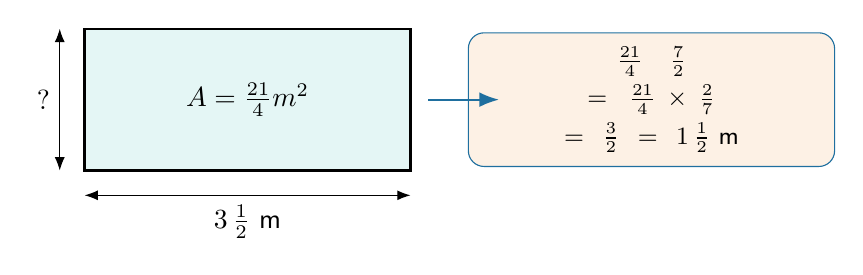
\begin{tikzpicture}[scale=0.9]
		\draw[thick, fill=iiiepeAqua!12] (0,0) rectangle (4.6,2.0);
		\draw[Latex-Latex] (0,-0.35) -- (4.6,-0.35) node[midway,below] {$3\,\frac12$ m};
		\draw[Latex-Latex] (-0.35,0) -- (-0.35,2.0) node[midway,left] {$?$};
		\node at (2.3,1.0) {$A=\frac{21}{4}\text{ m}^2$};
		\node[cajaOp, text width=4.3cm] at (8.0,1.0) {
			$\frac{21}{4}\signodiv\frac72$\\[1mm]
			$=\frac{21}{4}\times\frac27$\\[1mm]
			$=\frac32=1\,\frac12$ m
		};
		\draw[flechaProc] (4.85,1.0) -- (5.85,1.0);
	\end{tikzpicture}
	\caption{Situacion 06: obtener la medida faltante a partir del area.}
\end{figure}

\begin{figure}[H]
	\centering
	\resizebox{0.92\linewidth}{!}{%
	\RutaOperacionCinco
	{$20$ ha}
	{vender\\$8$}
	{restan\\$12$}
	{alquilar\\$9$}
	{quedan\\$3$}}
	\caption{Situacion 05: proceso encadenado de venta, resto, alquiler y saldo final.}
\end{figure}

\section{Evaluacion y retroalimentacion}

\subsection{Autoevaluacion del estudiante}

\begin{table}[H]
\centering
\caption{Autoevaluación alineada con la Sesión 03}
\label{tab:autoevaluacion-sesion03}

\small
\renewcommand{\arraystretch}{1.45}
\setlength{\tabcolsep}{5pt}
\rowcolors{2}{gray!10}{white}

\begin{tabularx}{\textwidth}{@{}
>{\raggedright\arraybackslash}X
>{\centering\arraybackslash}p{0.12\textwidth}
>{\centering\arraybackslash}p{0.14\textwidth}
>{\centering\arraybackslash}p{0.14\textwidth}
>{\centering\arraybackslash}p{0.07\textwidth}
@{}}
\toprule
\textbf{Indicador} &
\makecell{\textbf{Logrado}\\\textbf{(3)}} &
\makecell{\textbf{En proceso}\\\textbf{(2)}} &
\makecell{\textbf{No logrado}\\\textbf{(1)}} &
\textbf{Valor} \\
\midrule

Realizo multiplicaciones de fracciones de manera eficiente utilizando el algoritmo aprendido. 
& $\square$ & $\square$ & $\square$ & \\

Realizo divisiones de fracciones utilizando de forma correcta el recíproco. 
& $\square$ & $\square$ & $\square$ & \\

Identifico correctamente la operación para resolver un problema. 
& $\square$ & $\square$ & $\square$ & \\

Convierto enteros y fracciones mixtas antes de operar cuando es necesario. 
& $\square$ & $\square$ & $\square$ & \\

Simplifico e interpreto la respuesta según el contexto del problema. 
& $\square$ & $\square$ & $\square$ & \\

\bottomrule
\end{tabularx}

\end{table}

\subsection{Criterios para retroalimentar}

\begin{itemize}
	\item Si el estudiante cree que toda multiplicacion aumenta, se revisa una representacion de area para mostrar que una fraccion de una fraccion puede ser menor.
	\item Si divide sin usar reciproco, se le solicita escribir verbalmente la pregunta: ``cuantas partes de este tamano caben en la cantidad inicial?''.
	\item Si invierte la primera fraccion, se marca el dividendo y el divisor con colores distintos antes de transformar la operacion.
	\item Si opera fracciones mixtas como si fueran enteros separados, se exige el paso previo de conversion a impropia.
	\item Si omite unidades, se revisa si el resultado representa litros, metros, hectareas, botellas, vasos, bolsas o dinero.
\end{itemize}

\section{Conclusion}

La actualizacion de la actividad de la Sesion 03 organiza la multiplicacion y division con fracciones como una secuencia didactica completa: primero se recuperan conocimientos previos, despues se explica el sentido de las operaciones, luego se practica con ejercicios graduados, se evalua mediante situaciones contextualizadas y se cierra con retroalimentacion. Esta estructura responde a los lineamientos institucionales revisados y evita que el producto se limite a una hoja de respuestas.

El criterio central es que multiplicar fracciones significa tomar partes de partes, mientras que dividir entre fracciones significa identificar cuantos grupos fraccionarios caben en una cantidad. Por eso, cada solucion debe mostrar estrategia, transformacion, calculo, simplificacion e interpretacion. Cuando el estudiante puede explicar por que usa el reciproco, como convierte mixtas, que representa el producto y que unidad tiene la respuesta final, el aprendizaje deja de ser memoristico y se vuelve transferible a problemas de medida, consumo, area, reparto y capacidad.

% FIN DEL DOCUMENTO
\end{document}
